\section{HDBSCAN} \label{sec:HDBSCAN}

\gls{HDBSCAN} is an clustering algorithm proposed by \textcite{campello_hierarchical_2015, hutchison_density-based_2013}. It is a novel version of \gls{DBSCAN} but executed with varying values of $\varepsilon$ \autocite{hutchison_density-based_2013}. Thus not one specific threshold is used to define the clusters, but instead clusters of varying densities are extracted based on their stability over epsilon \autocite{mcinnes_hdbscan_2017}. The version of \gls{HDBSCAN} used in this project is the accelerated implementation by the \textbf{hdbscan} package version 0.8.26 of \textcite{mcinnes_accelerated_2017} (\autoref{fig:Clustering_Pipeline} \textsf{\textbf{F}}).

Since there is, to my best knowledge, no submission using \gls{HDBSCAN} for a usecase similar to the one proposed in this project, most settings for \gls{HDBSCAN} were selected by parameter exploration, graphical comparisons and reasonable assumptions. For the selection of all settings the \href{https://hdbscan.readthedocs.io/en/latest/api.html}{API} was used as backup \autocite{mcinnes_hdbscan_2017}. 

To capture, in the best case, even genomes with single \glspl{SNP} at rare appearing positions in their own clusters \colorbox{backcolour}{min\_cluster\_size=2} and \colorbox{backcolour}{min\_samples=1} setting was used as default in the project. These settings are in both cases the smallest values possible, to declare as least points as possible as noise. Setting the \gls{UMAP} parameters to focus on the global structure, while cluster as fine as possible might sound contradictory and is therefore discussed in \autoref{sec:Dimension_Reduction}. The default \colorbox{backcolour}{metric='euclidean'} setting was used for all following executions of \gls{HDBSCAN}, with an exception on the precalculated runs, to approximate the use of cosine distance metric as described in \autoref{sec:Normalization}. Therefore matrix $\mathbf{X}_{\text{PCA}}$ and $\mathbf{Y}_{\text{UMAP}}$ have to be L2-normalized as described in \autoref{sec:Normalization} (\autoref{eq:l2_func_x} and \autoref{eq:l2_func_y}). For calculation of the linkage matrix $\mathbf{L}$ standard \gls{HDBSCAN} without $\varepsilon$ was used.

\autoref{eq:HDB} to \autoref{eq:HDB_link_X} demonstrate the use of \gls{HDBSCAN} to calculate the linkage matrix $\mathbf{L}_{\text{PCA}}$ with matrix $\mathbf{X}_{\text{L2}}$ of \autoref{fig:Clustering_Pipeline} pathway \textsf{\textbf{1}} and was performed in the same way for $\mathbf{L}_{\text{UMAP}}$ with $\mathbf{Y}_{\text{L2}}$ of \autoref{fig:Clustering_Pipeline} pathway \textsf{\textbf{2}} \autocite{mcinnes_hdbscan_2017, gower_minimum_1969}.

\begin{empheq}{alignat = -1}
    &\mathbf{X}_{\text{L2}} &&= \text{NORMALIZE}_{\text{L2}}(\mathbf{X}_{\text{PCA}})\label{eq:l2_func_x}\\
    &\mathbf{Y}_{\text{L2}} &&= \text{NORMALIZE}_{\text{L2}}(\mathbf{Y}_{\text{UMAP}})\label{eq:l2_func_y}
\end{empheq}

\begin{empheq}{alignat = -1}
    &\mathbf{L}_{\text{PCA}} &&= \text{HDBSCAN}_{\text{Link}}(\mathbf{X}_{\text{L2}}, \text{min\_cluster\_size}, \text{min\_samples})\label{eq:HDB}\\
    &&&= \text{HDBSCAN}_{\text{Link}}(\mathbf{X}_{\text{L2}}, 2, 1) \label{eq:HDB_link_X}
\end{empheq}

By combining \gls{HDBSCAN} with \gls{DBSCAN} some of the disadvantages of using either of these methods can be overcome \autocite{mcinnes_hdbscan_2017, moulavi_density-based_2014}. Since \gls{DBSCAN} is a hierarchical clustering tool, it is dependent on a strict threshold for clustering. Points not included in this threshold value are omitted \autocite{ester_density-based_1996, schubert_dbscan_2017}. \gls{HDBSCAN} on the other hand tend to create micro-clusters in areas of high density \autocite{mcinnes_hdbscan_2017}. Using the hybrid approach proposed in \autocite{malzer_hybrid_2020} a threshold value $\varepsilon$ can be used to extract clusters but still use the method of \gls{HDBSCAN} instead of emitting other points. This method is useful when having a small cluster size value while still want to cluster high-density areas together \autocite{malzer_hybrid_2020}.

\begin{figure}[!hbt]
    \centering
    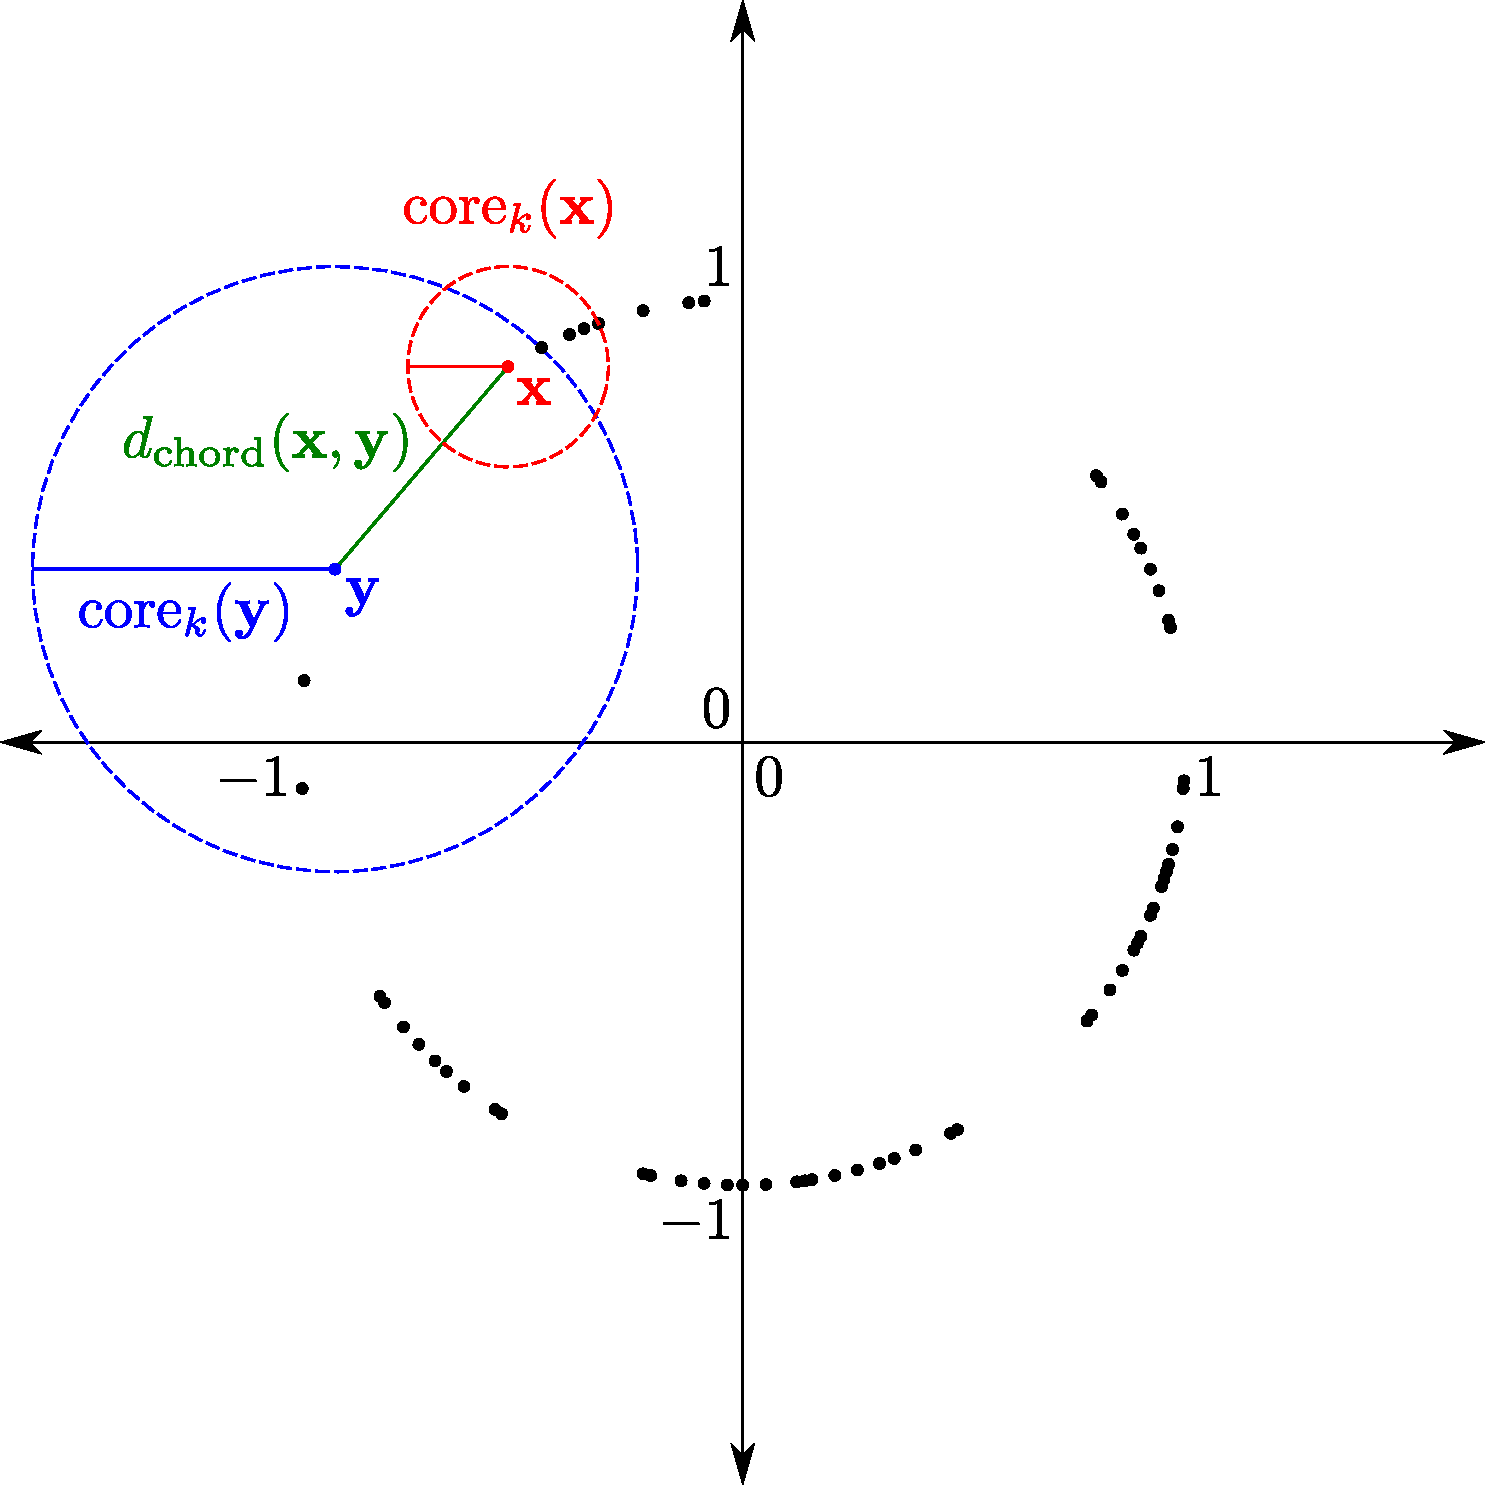
\includegraphics[width=\textwidth]{Graphics/HDB.pdf}
    \caption[]{\textbf{.}.}
    \label{fig:HDB}
\end{figure}

\begin{figure}[!hbt]
    \centering
    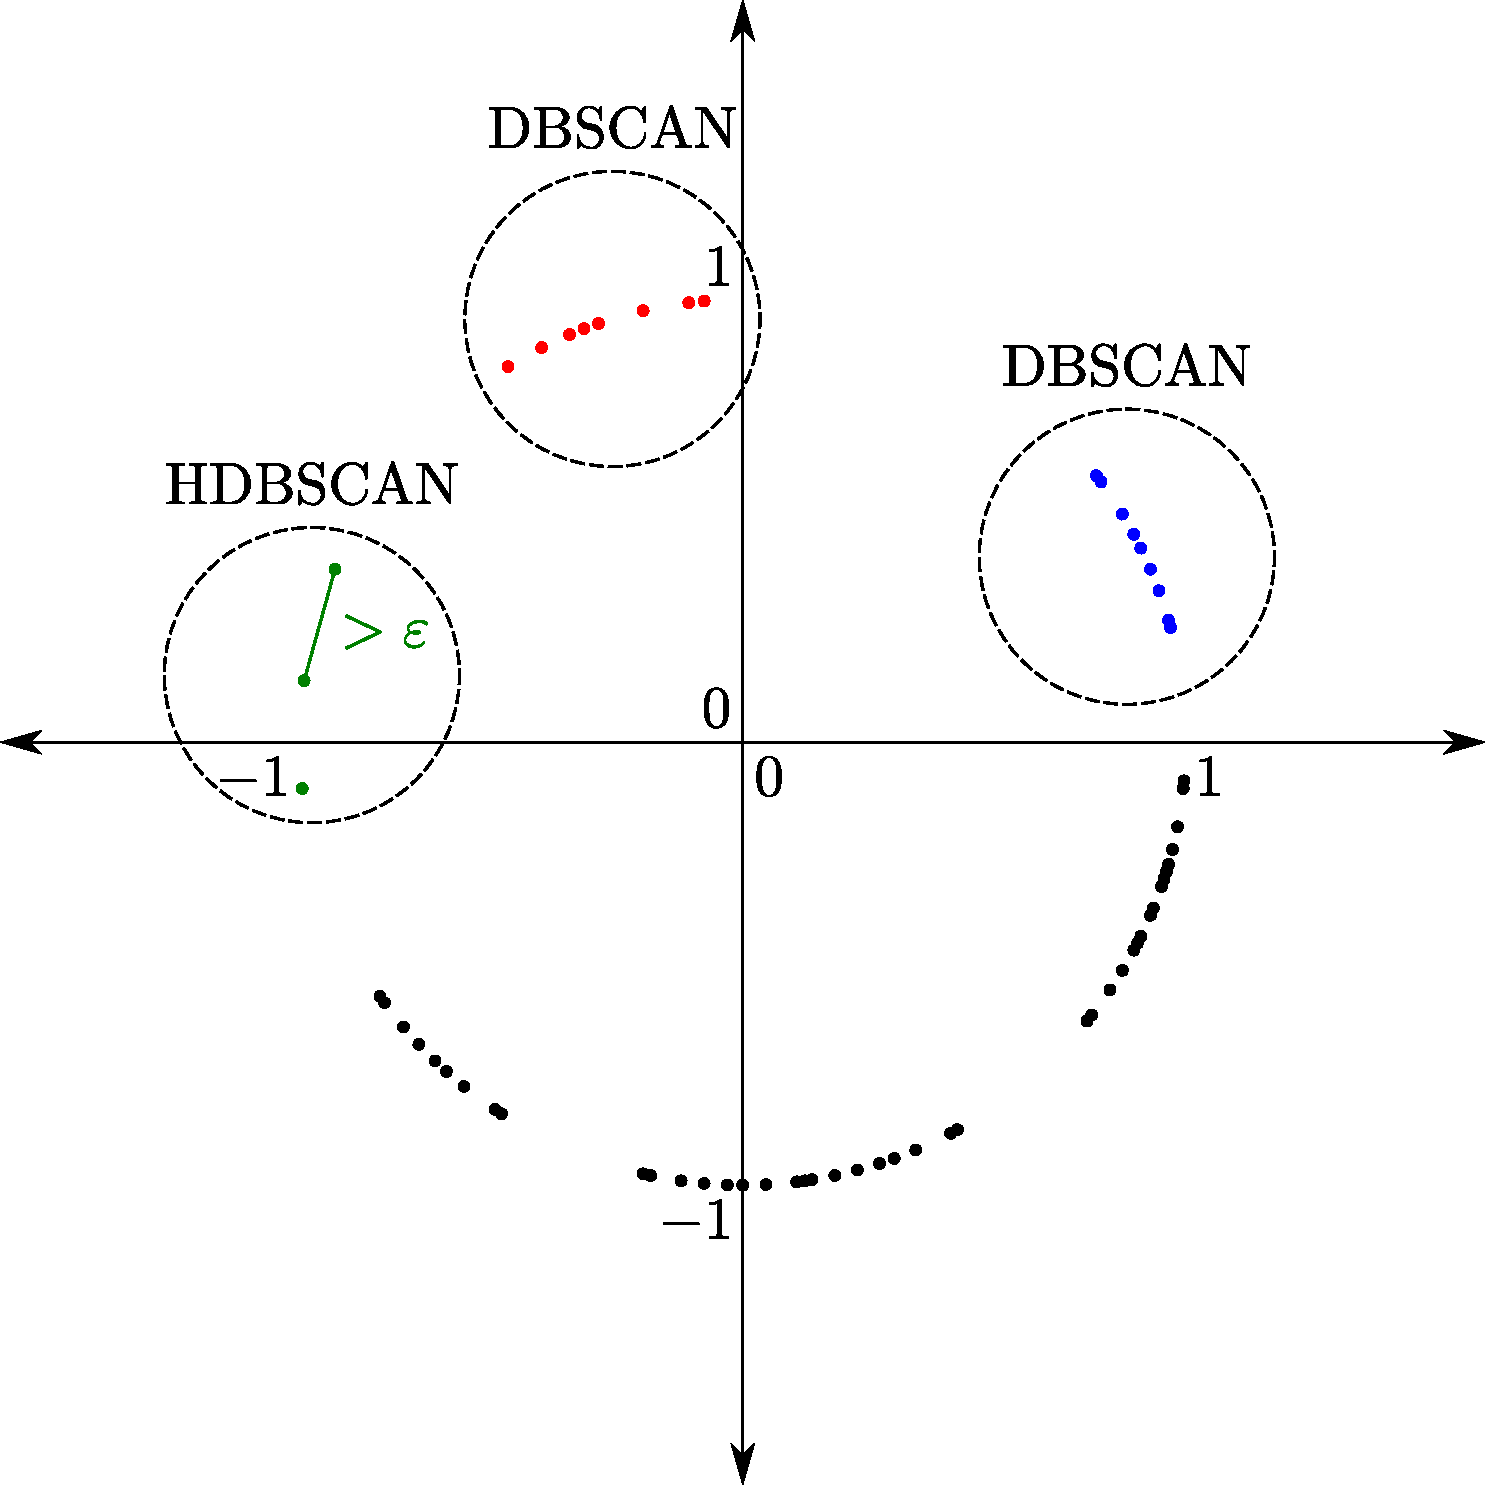
\includegraphics[width=\textwidth]{Graphics/Hybrid.pdf}
    \caption[]{\textbf{.}.}
    \label{fig:Hybrid}
\end{figure}

To find an appropriate value for $\varepsilon$ two different methods were used and compared (\autoref{fig:Clustering_Pipeline} pathway \textsf{\textbf{3}} and \textsf{\textbf{4}}. Using the first method, the \gls{DBCV} exploration in \autoref{fig:Clustering_Pipeline} \textsf{\textbf{G}}, execution of \gls{HDBSCAN} was repeated with different settings for $\varepsilon$ and compared by the \gls{DBCV} to find the value of $\varepsilon$ that maximizes the \gls{DBCV} \autocite{moulavi_density-based_2014}. For these repeated executions of \gls{HDBSCAN}, \colorbox{backcolour}{gen\_min\_span\_tree=True} setting was also necessary, to be able to calculate the \gls{DBCV}, by the minimum spanning tree (\autoref{eq:DBCV_X}) \autocite{moulavi_density-based_2014, gower_minimum_1969}. The exploration was executed for $\mathbf{X}_{\text{L2}}$ and $\mathbf{Y}_{\text{L2}}$ to find the optimal $\varepsilon_{\text{PCA}}$ and $\varepsilon_{\text{UMAP}}$.

\begin{empheq}{alignat = -1}
    &\max_{\substack{0 \leq \varepsilon}} \left(\text{HDBSCAN}_{\text{DBCV}}(\mathbf{X}_{\text{L2}}, 2, 1, \varepsilon)\right) = \text{HDBSCAN}_{\text{DBCV}}(\mathbf{X}_{\text{L2}}, 2, 1, \varepsilon') \Rightarrow \varepsilon' = \varepsilon_{\text{PCA}} \label{eq:DBCV_X}
\end{empheq}

Using the second method the optimal value for $\varepsilon_{\text{UMAP'}}$ and $\varepsilon_{\text{PCA'}}$ were calculated using the Kneedle algorithm \autoref{sec:Kneedle} \autocite{halko_finding_2010}.

With the optimal values for $\varepsilon$ found by \gls{DBCV} exploration and the Kneedle Algorithm, as well as with the matrix for the \gls{UMAP} settings and the one for the \gls{PCA} settings, \gls{HDBSCAN} with the hybrid clustering setting was executed four times. Each execution results in the mathematical sequence of cluster names $N$ related to the sequence of genomic sequences $S$ (\autoref{eq:HDB_cluster_PK} to \autoref{eq:HDB_cluster_UD}) (\autoref{fig:Clustering_Pipeline} \textsf{\textbf{H}}) \autocite{mcinnes_hdbscan_2017, malzer_hybrid_2020}. To sum it up, with the \acrshort{UMAP}/\acrshort{DBCV} method, the cluster name of the first genomic sequence of $S$ is the first element of mathematical sequence $N_{\text{UMAP}}$. 

\begin{empheq}{alignat = -1}
    &N_{\text{PCA}} &&= \text{HDBSCAN}_{\text{Hybrid}}(\mathbf{X}_{\text{L2}}, 2, 1, \varepsilon_{\text{PCA}}) \label{eq:HDB_cluster_PK}\\
    &N_{\text{UMAP}} &&= \text{HDBSCAN}_{\text{Hybrid}}(\mathbf{Y}_{\text{L2}}, 2, 1, \varepsilon_{\text{UMAP}}) \label{eq:HDB_cluster_UK}\\
    &N_{\text{PCA'}} &&= \text{HDBSCAN}_{\text{Hybrid}}(\mathbf{X}_{\text{L2}}, 2, 1, \varepsilon_{\text{PCA'}}) \label{eq:HDB_cluster_PD}\\
    &N_{\text{UMAP'}} &&= \text{HDBSCAN}_{\text{Hybrid}}(\mathbf{Y}_{\text{L2}}, 2, 1, \varepsilon_{\text{UMAP'}}) \label{eq:HDB_cluster_UD}
\end{empheq}

The parameters used in this project with settings varying from the default are listed below. All available settings can be fount in the \href{https://hdbscan.readthedocs.io/en/latest/api.html}{API}.

\begin{leftbar}
    \textbf{hdbscan.HDBSCAN}
    \begin{nstabbing}
        \qquad\qquad\qquad\qquad\qquad\quad\=\kill

        min\_cluster\_size \> [min. size of a cluster (default: 5)]\\
        
        min\_samples \> [conservativeness of the clustering (default: None)]\\
        
        cluster\_selection\_epsilon \> [merge clusters below the threshold (default: 0.0)]\\
        
        gen\_min\_span\_tree \> [generate the minimum spanning tree (default: False)]\\
        
        metric \> [metric to use for clustering (default: euclidean)]
        %alpha \> (default: 1.0)
    \end{nstabbing}
\end{leftbar}

%Clustering
%DBCV mehr als 50dims abkacken bla
%Metrik
%Hybrid selection
%Needle
%Linkage matrix